\section{Problem statement}
\label{bended-plate:sec:problem-statement}

An initially horizontal and unloaded quadratic plate of $a = \qty{2}{\metre}
    \times b = \qty{2}{\metre}$ with a thickness of $t = \qty{0.1}{\metre} =
    \qty{10}{\centi\metre}$ is only held at one edge and is subjected at the
opposite edge with a static point load of $F = \qty{100}{\kilo\newton}$
directed upwards. This test setup can be seen in
\autoref{bended-plate:fig:setup}. The material behaviour is purely
linear-elastic and the corresponding parameters can be found in
\autoref{bended-plate:material-parameters}.

The deflection of the plate at the loaded edge is to be determined as a
simulation result.

This problem is closely related to classical beam bending theory for a
cantilever (fully fixed at one end) with a point load at the (opposite) free
end. This conveniently provides an analytical solution
(\autoref{bended-plate:sec:analytical-solution}) against which the numerical
results can be checked (\autoref{bended-plate:sec:moose} and
\autoref{bended-plate:sec:plaxis3D}). With this problem setup, the plate may be
modelled using volume elements or shell elements.

\begin{table}[htbp]
    \centering
    \caption{Material parameters}
    \label{bended-plate:material-parameters}
    \begin{tabularx}{\textwidth}{XYY}

        \hline

        Property              & Physical unit                                         & Value      \\

        \hline

        Youngs modulus $E$    & \si[per-mode = symbol]{\kilo\newton\per\square\metre} &
        \SI{1E6}{}                                                                                 \\

        Poisson's ratio $\nu$ & -                                                     & \SI{0.3}{} \\

        density $\rho$        & \si[per-mode = symbol]{\kilogram\per\cubic\metre}     & \SI{0}{}
        \\

        \hline
    \end{tabularx}
\end{table}

\begin{figure}[htbp]
    \centering
    \begin{tikzpicture}

        \def\Dimline[#1][#2][#3][#4]{
            \begin{scope}[>=latex] % redef arrow for dimension lines
                \draw let \p1=#1, \p2=#2, \n0={veclen(\x2-\x1,\y2-\y1)} in [|<->|,
                        decoration={markings, % switch on markings
                                mark=at position .5 with {\node[#3] at (0,0) {#4};},
                            },
                        postaction=decorate] #1 -- #2 ;
            \end{scope}
        }

        % this image has been generated using Blender writing a SVG
        % using the "Freestyle SVG Exporter". The SVG is minimized
        % using third-party tools and finally converted to PDF using
        % Inkscape.
        \node[inner sep=0pt] (ch-stresses) at (0,0) {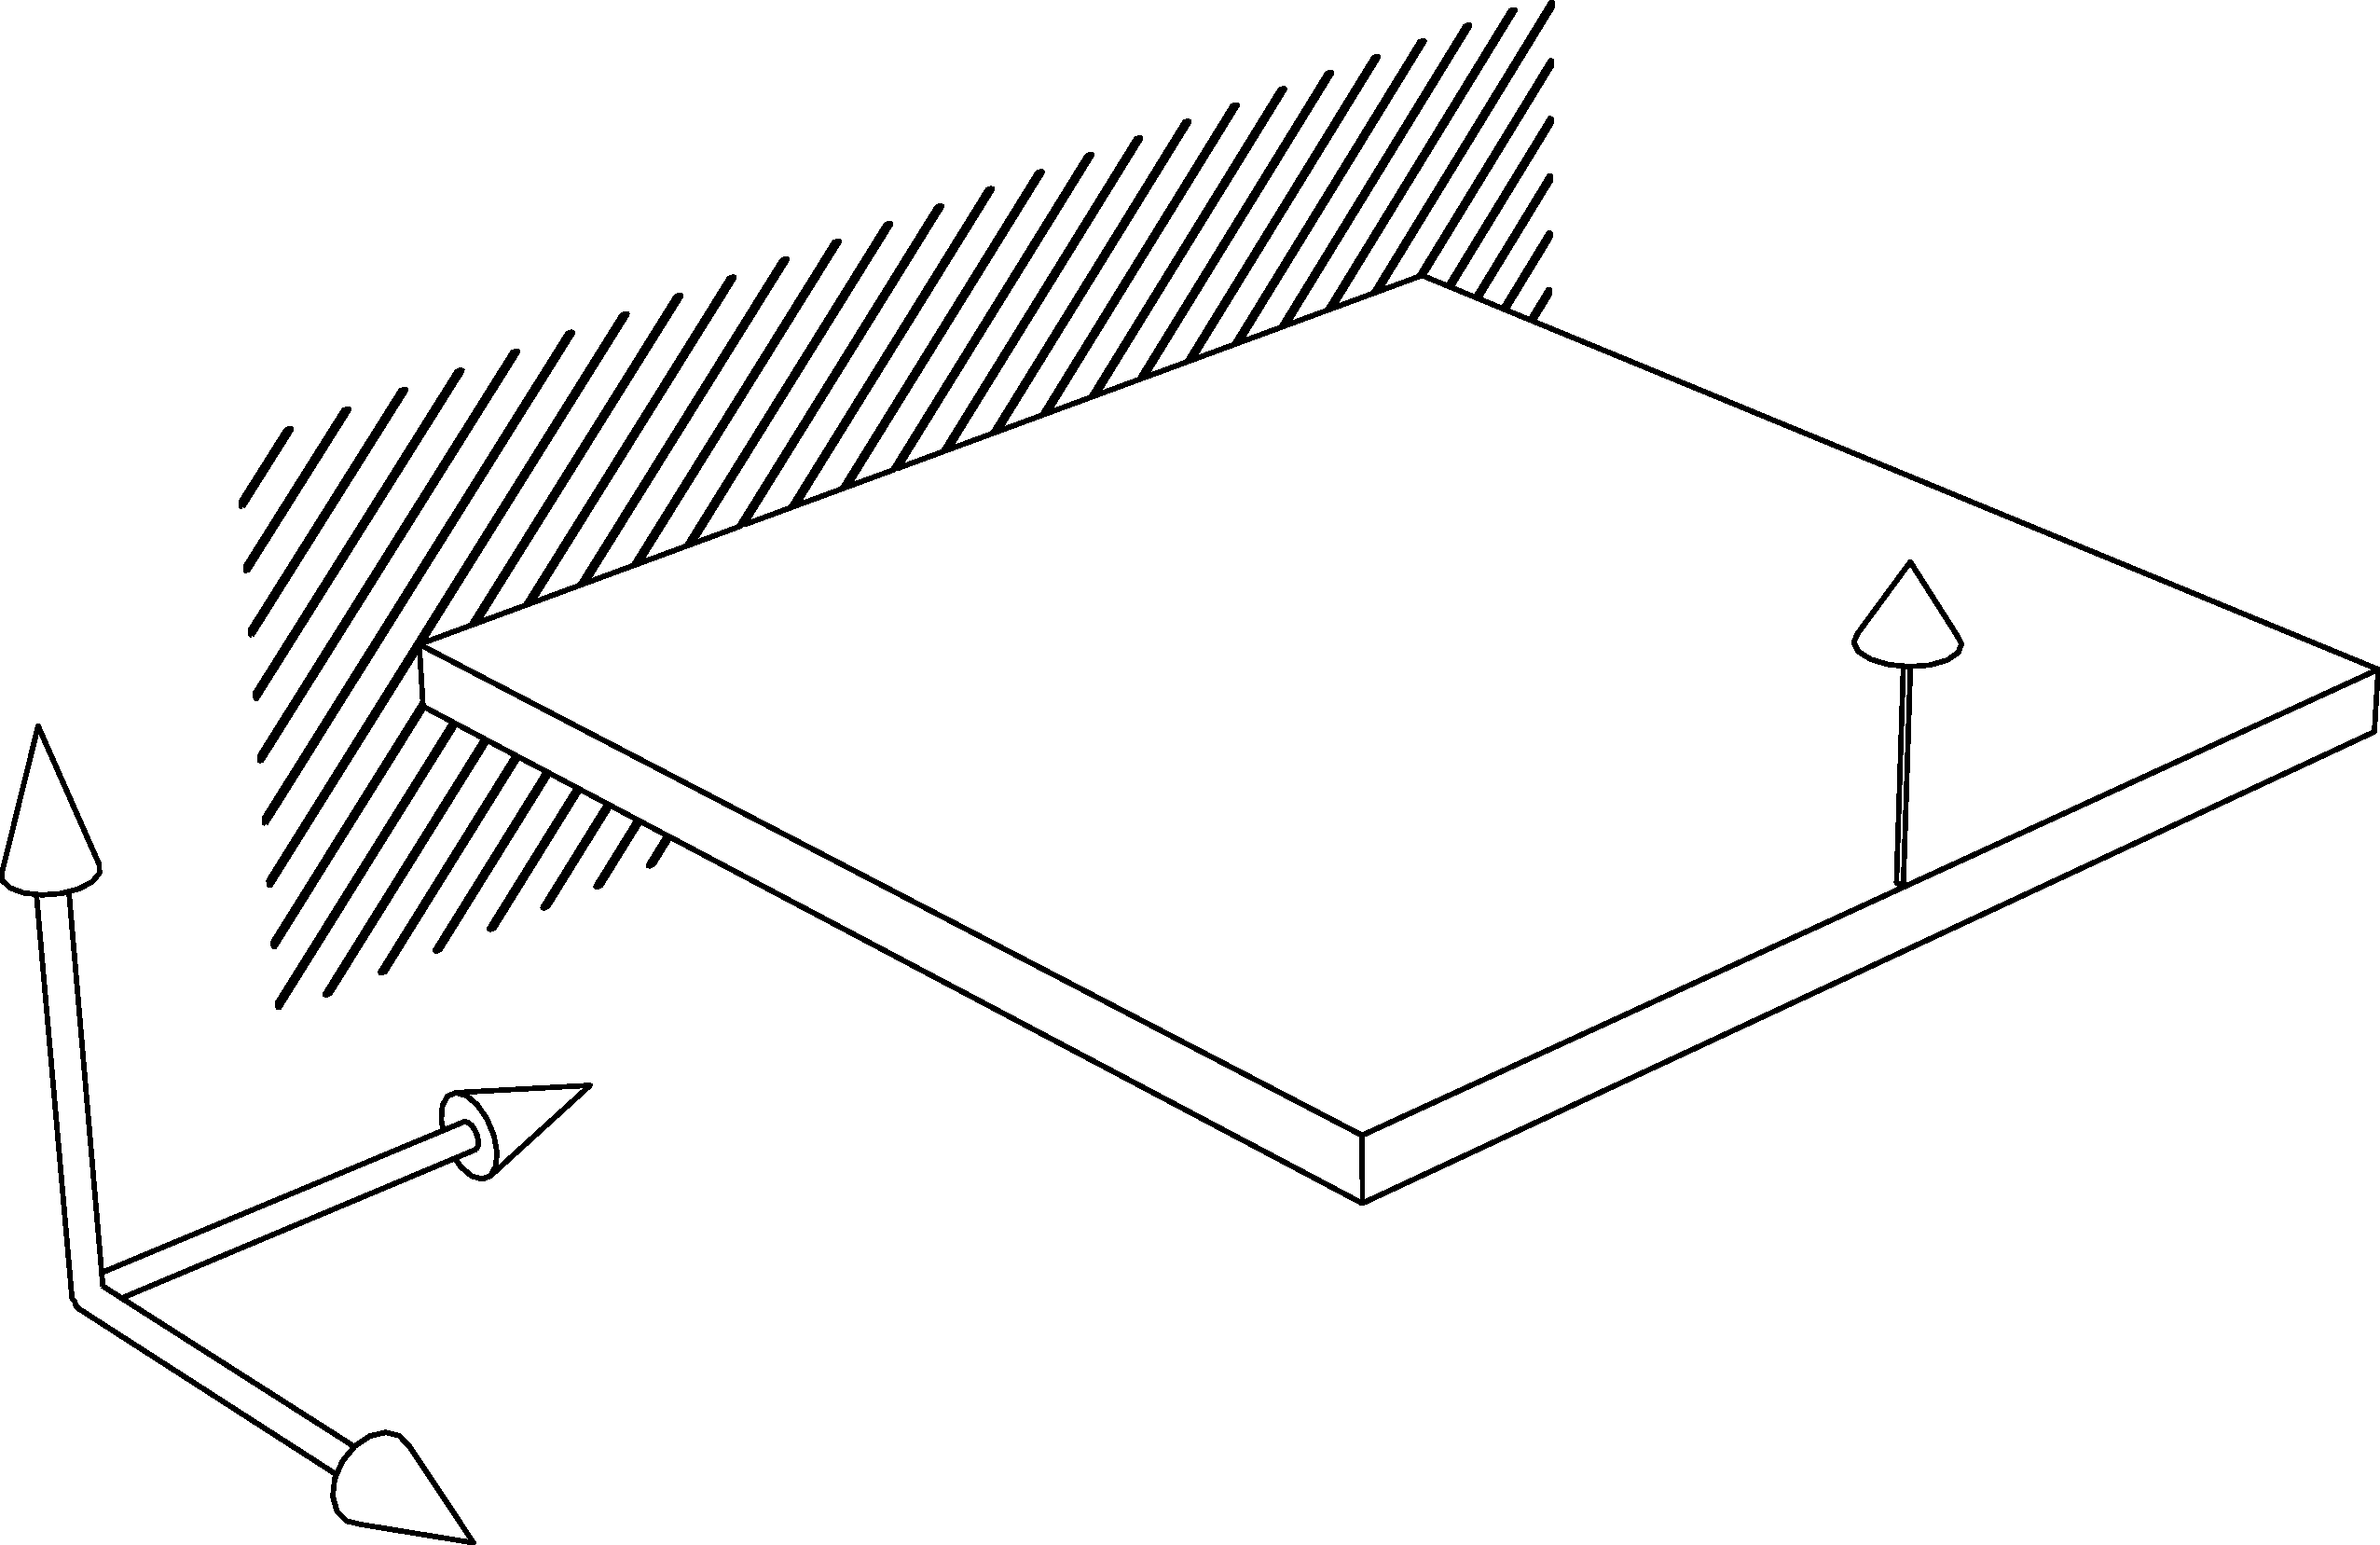
\includegraphics[width=0.4\linewidth]{\currfiledir/bended-plate.blend-min.svg.pdf}};

        \node[] at (-2.8,-2.2) {x};
        \node[] at (-2.0,-1.5) {y};
        \node[] at (-3.7,-0.0) {z};

        \node[rotate=+16] at (-2.4,+1.4) {fixed};

        \node[left] at (+2.0,+0.6) {$F = \qty{100}{\kilo\newton}$};

        \node[] at (+0.6,-1.4) (A) {};
        \node[] at (+3.5,-0.0) (B) {};
        \node[] at (+1.0,+1.0) (C) {};
        \Dimline[($(A)+(+0.1,-0.1)$)][($(B)+(+0.1,-0.1)$)][below right][\qty{2}{\metre}];
        \Dimline[($(C)+(-0.2,+0.6)$)][($(B)+(+0.1,+0.5)$)][above right][\qty{2}{\metre}];
        \Dimline[($(B)+(+0.5,+0.1)$)][($(B)+(+0.5,+0.3)$)][right][\qty{0.1}{\metre}];

    \end{tikzpicture}
    \caption{Setup of the bended plate test}
    \label{bended-plate:fig:setup}
\end{figure}

\section{Analytical solution}
\label{bended-plate:sec:analytical-solution}

Neglecting geometrical non-linearity, the well-known analytical solution for
the deflection is given in \autoref{bended-plate:analytical-solution}.

\begin{equation}
    \label{bended-plate:analytical-solution}
    u_z = F \cdot \frac{a ^ 3}{3EI} = \qty{1.6}{\metre}
\end{equation}

\begin{samepage}
    with:
    \begin{description}
        \item[$u_{z}$] vertical deflection at the point load to be estimated.
        \item[$F$] point load (\qty{100}{\kilo\newton})
        \item[$a$] size of the plate (\qty{2}{\metre})
        \item[$E$] Young's modulus (\qty[per-mode = symbol]{1E6}{\kilo\newton\per\square\metre}; see \autoref{bended-plate:material-parameters})
        \item[$I$] Second moment of area, for this geometry $I = \frac{b \cdot t^3}{12} = \frac{\qty{2}{\metre} \cdot (\qty{0.1}{\metre})^3}{12} = 0.0001\overline{6} \qty{}{\metre}^4 $
    \end{description}
\end{samepage}

\section{Moose}
\label{bended-plate:sec:moose}

In \autoref{bended-plate:moose-results} the deflection and some additional
metrics of selected Moose models for this problem is shown.

For this purely linear-elastic problem, the ‘NEWTON’ solver is used. The Moose
input files for this model are attached to this document by the name of
‘bended-plate.i’.

%\fileattachment{\currfiledir/bended-plate.i}{bended-plate.i}

\begin{table}[htbp]
    \centering
    \caption{Resulting deflection for selected Moose models (geometrical non-linearity neglected)}
    \label{bended-plate:moose-results}
    \begin{tabularx}{\textwidth}{
            >{\hsize=0.3\hsize\linewidth=\hsize}X
            >{\hsize=0.2\hsize\linewidth=\hsize\hspace{-5pt}}Y
            >{\hsize=0.3\hsize\linewidth=\hsize\hspace{-5pt}}Y
            >{\hsize=0.2\hsize\linewidth=\hsize\hspace{-5pt}}Y}

        \hline

        Discretisation & deflection (\si{\metre}) & CPU-count / wall time
        (\si{\second}) & RAM (MB)                                                    \\

        \hline

        xxxxxxx TRI6   & \qty{}{}                 & 0 / \qty{}{}          & \qty{}{} \\

        xxxxxxx TET10  & \qty{}{}                 & 0 / \qty{}{}          & \qty{}{} \\

        xxxxxxx TET10  & \qty{}{}                 & 0 / \qty{}{}          & \qty{}{} \\

        \hline
    \end{tabularx}
\end{table}

\section{Plaxis 3D}
\label{bended-plate:sec:plaxis3D}

\autoref{bended-plate:plaxis-results}

\begin{table}[htbp]
    \centering
    \caption{Resulting deflection for selected Plaxis models (geometrical non-linearity neglected)}
    \label{bended-plate:plaxis-results}
    \begin{tabularx}{\textwidth}{
            >{\hsize=0.3\hsize\linewidth=\hsize}X
            >{\hsize=0.2\hsize\linewidth=\hsize\hspace{-5pt}}Y
            >{\hsize=0.3\hsize\linewidth=\hsize\hspace{-5pt}}Y
            >{\hsize=0.2\hsize\linewidth=\hsize\hspace{-5pt}}Y}

        \hline

        Discretisation & deflection (\si{\metre}) & CPU-count / wall time
        (\si{\second}) & RAM (MB)                                                    \\

        \hline

        xxxxxxx TRI6   & \qty{}{}                 & 0 / \qty{}{}          & \qty{}{} \\

        xxxxxxx TET10  & \qty{}{}                 & 0 / \qty{}{}          & \qty{}{} \\

        xxxxxxx TET10  & \qty{}{}                 & 0 / \qty{}{}          & \qty{}{} \\

        \hline
    \end{tabularx}
\end{table}